%!/usr/bin/env pdflatex
%-*- coding: utf-8 -*-
%@author : Romain Graux
%@date : 2022 June 06, 14:36:11
%@last modified : 2022 June 16, 17:06:52

\chapter{Appendix}

\begin{figure}
    \centering
    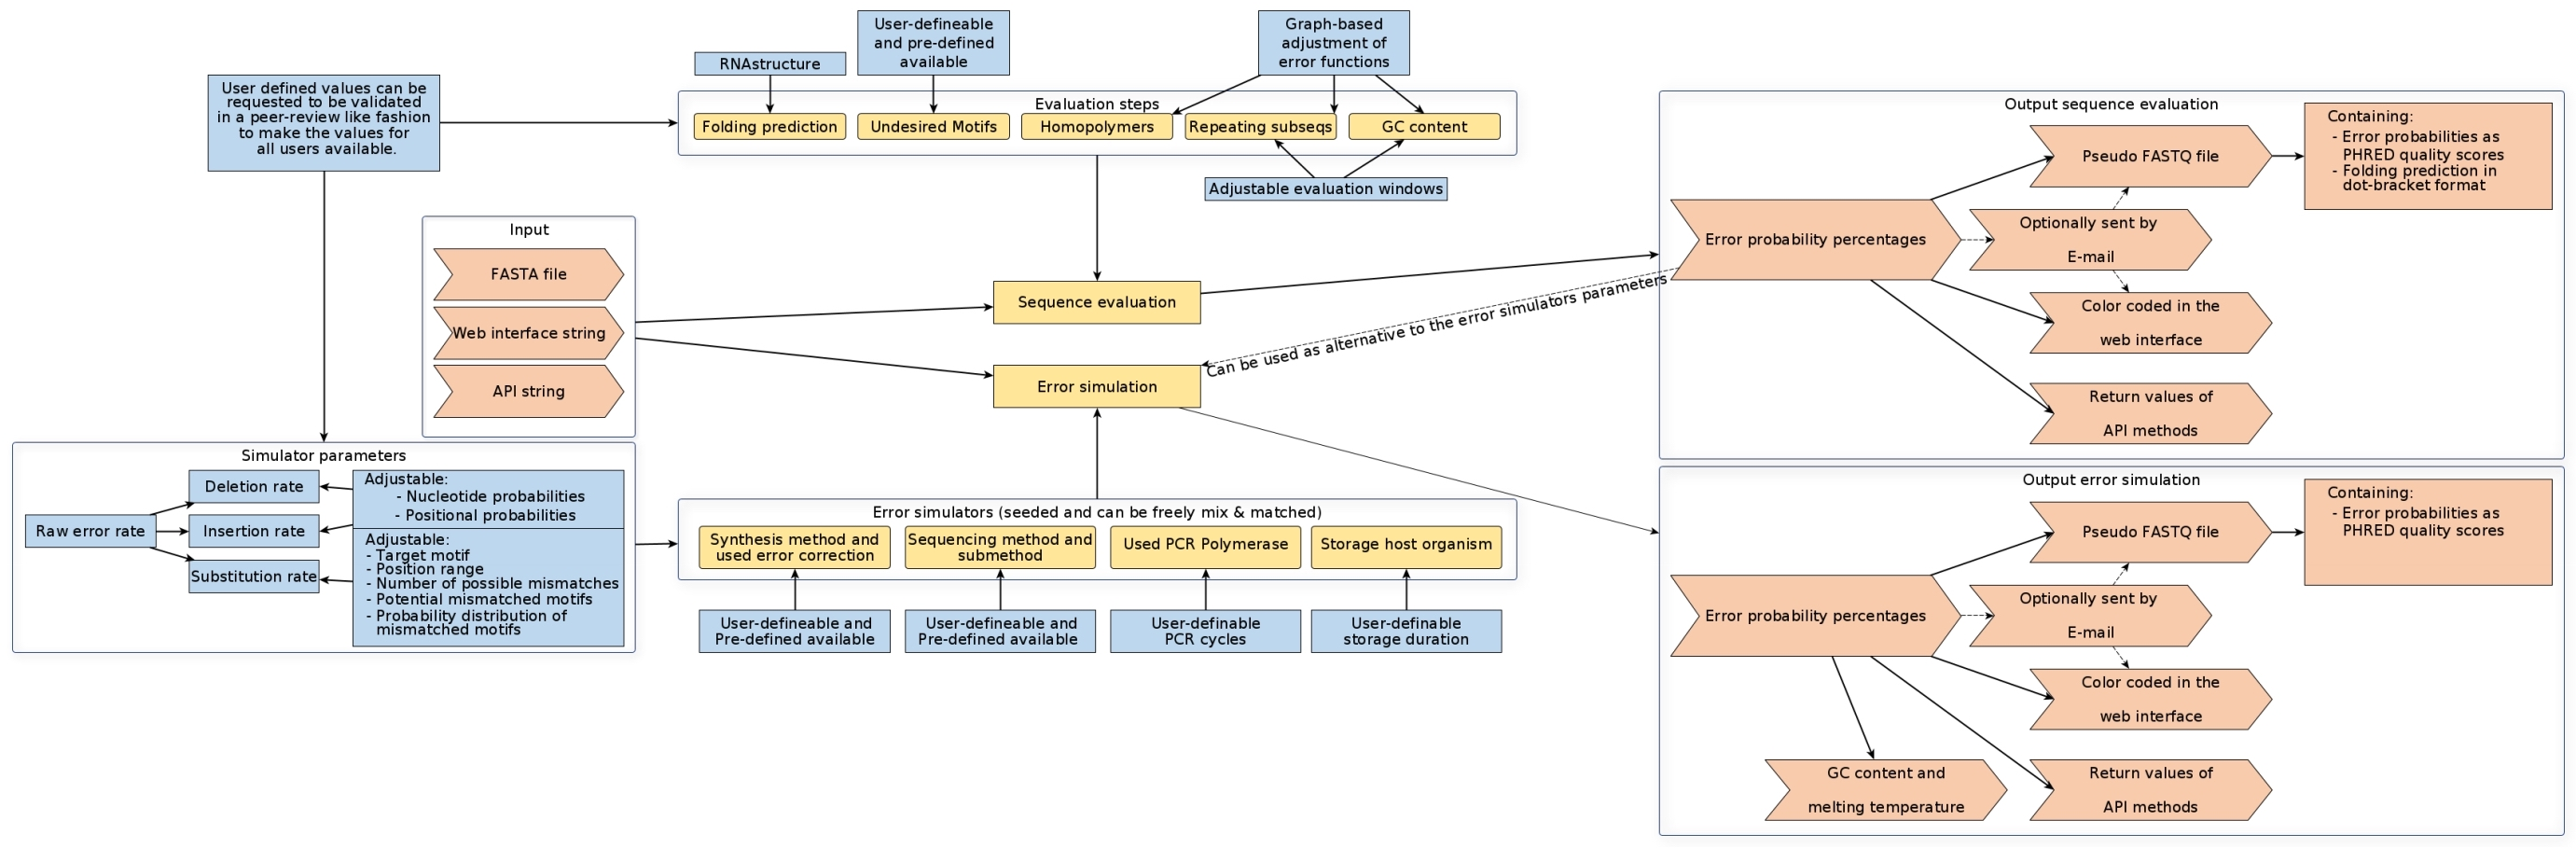
\includegraphics[width=\textwidth]{mesa_workflow.jpg}
    \caption{Mesa workflow}
    \label{fig:mesa_workflow}
\end{figure}

% \lstinputlisting[language=yaml, caption={Default parameters for MESA simulator}]{docs/code/mesa.yaml}

\begin{figure}
    \centering
    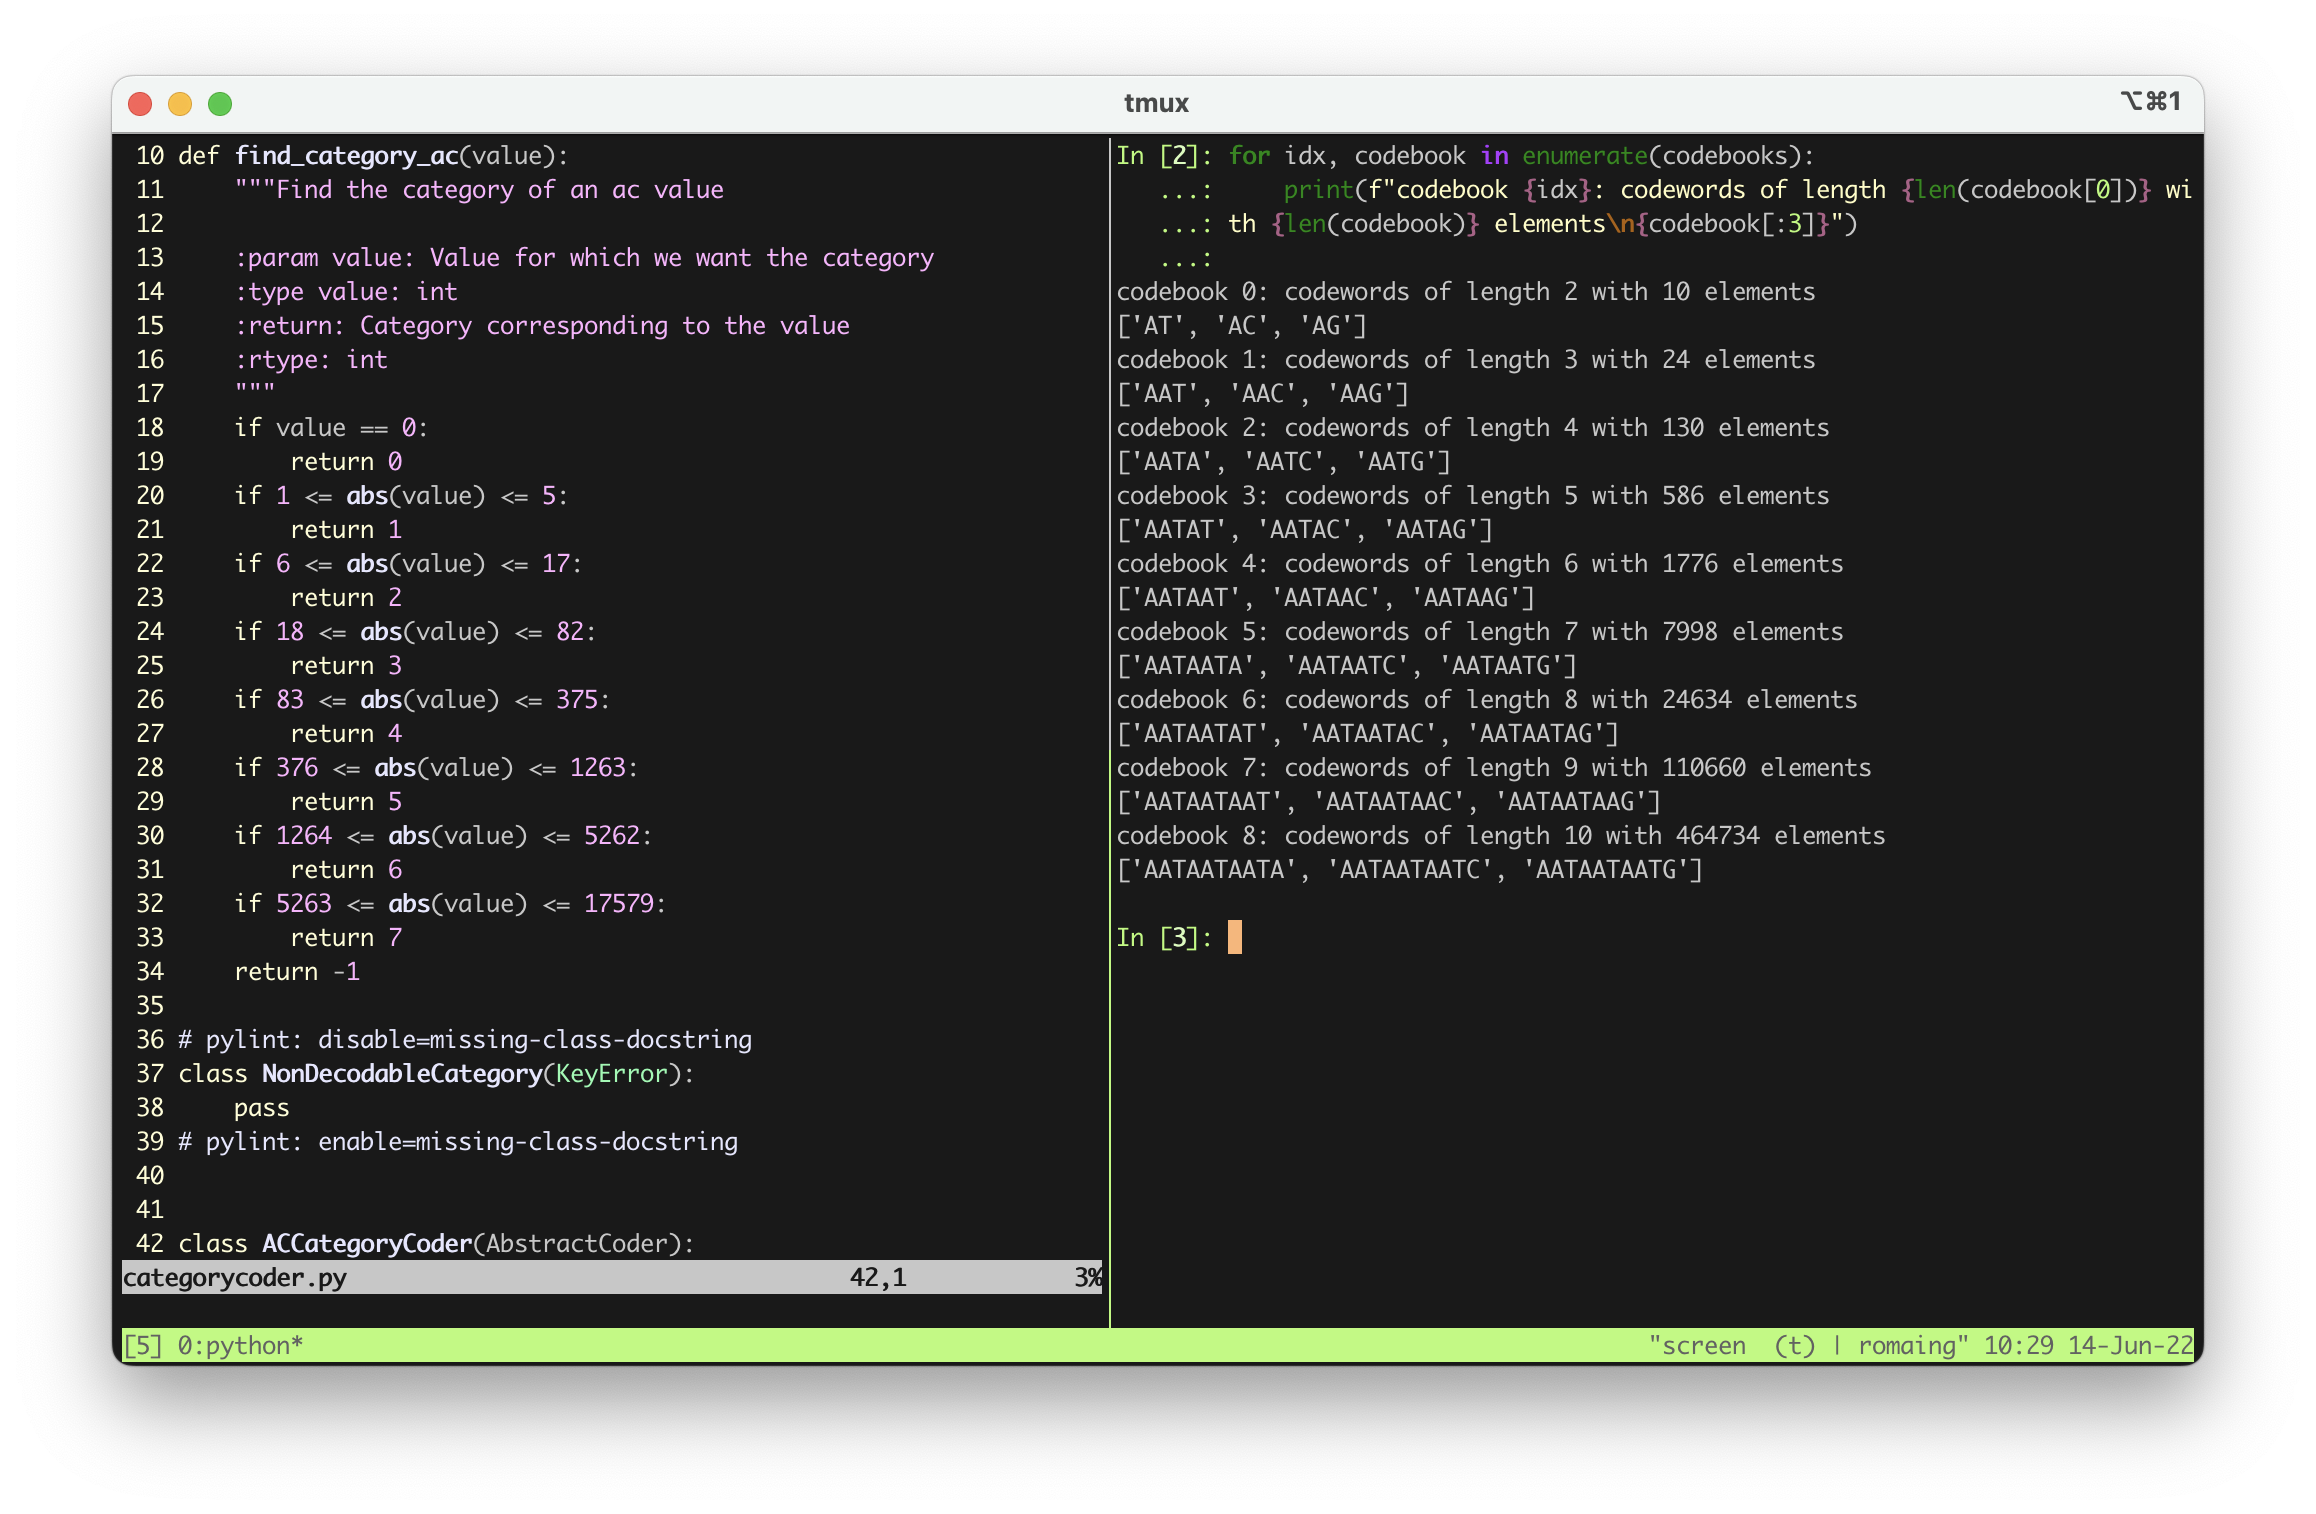
\includegraphics[width=\textwidth]{codebooks}
    \caption{The ranges for the AC coefficients categories and the codebooks associated used by the JPEG DNA codec}
    \label{fig:codebooks}
\end{figure}

\begin{figure}
    \begin{subfigure}{0.5\textwidth}
        \centering
        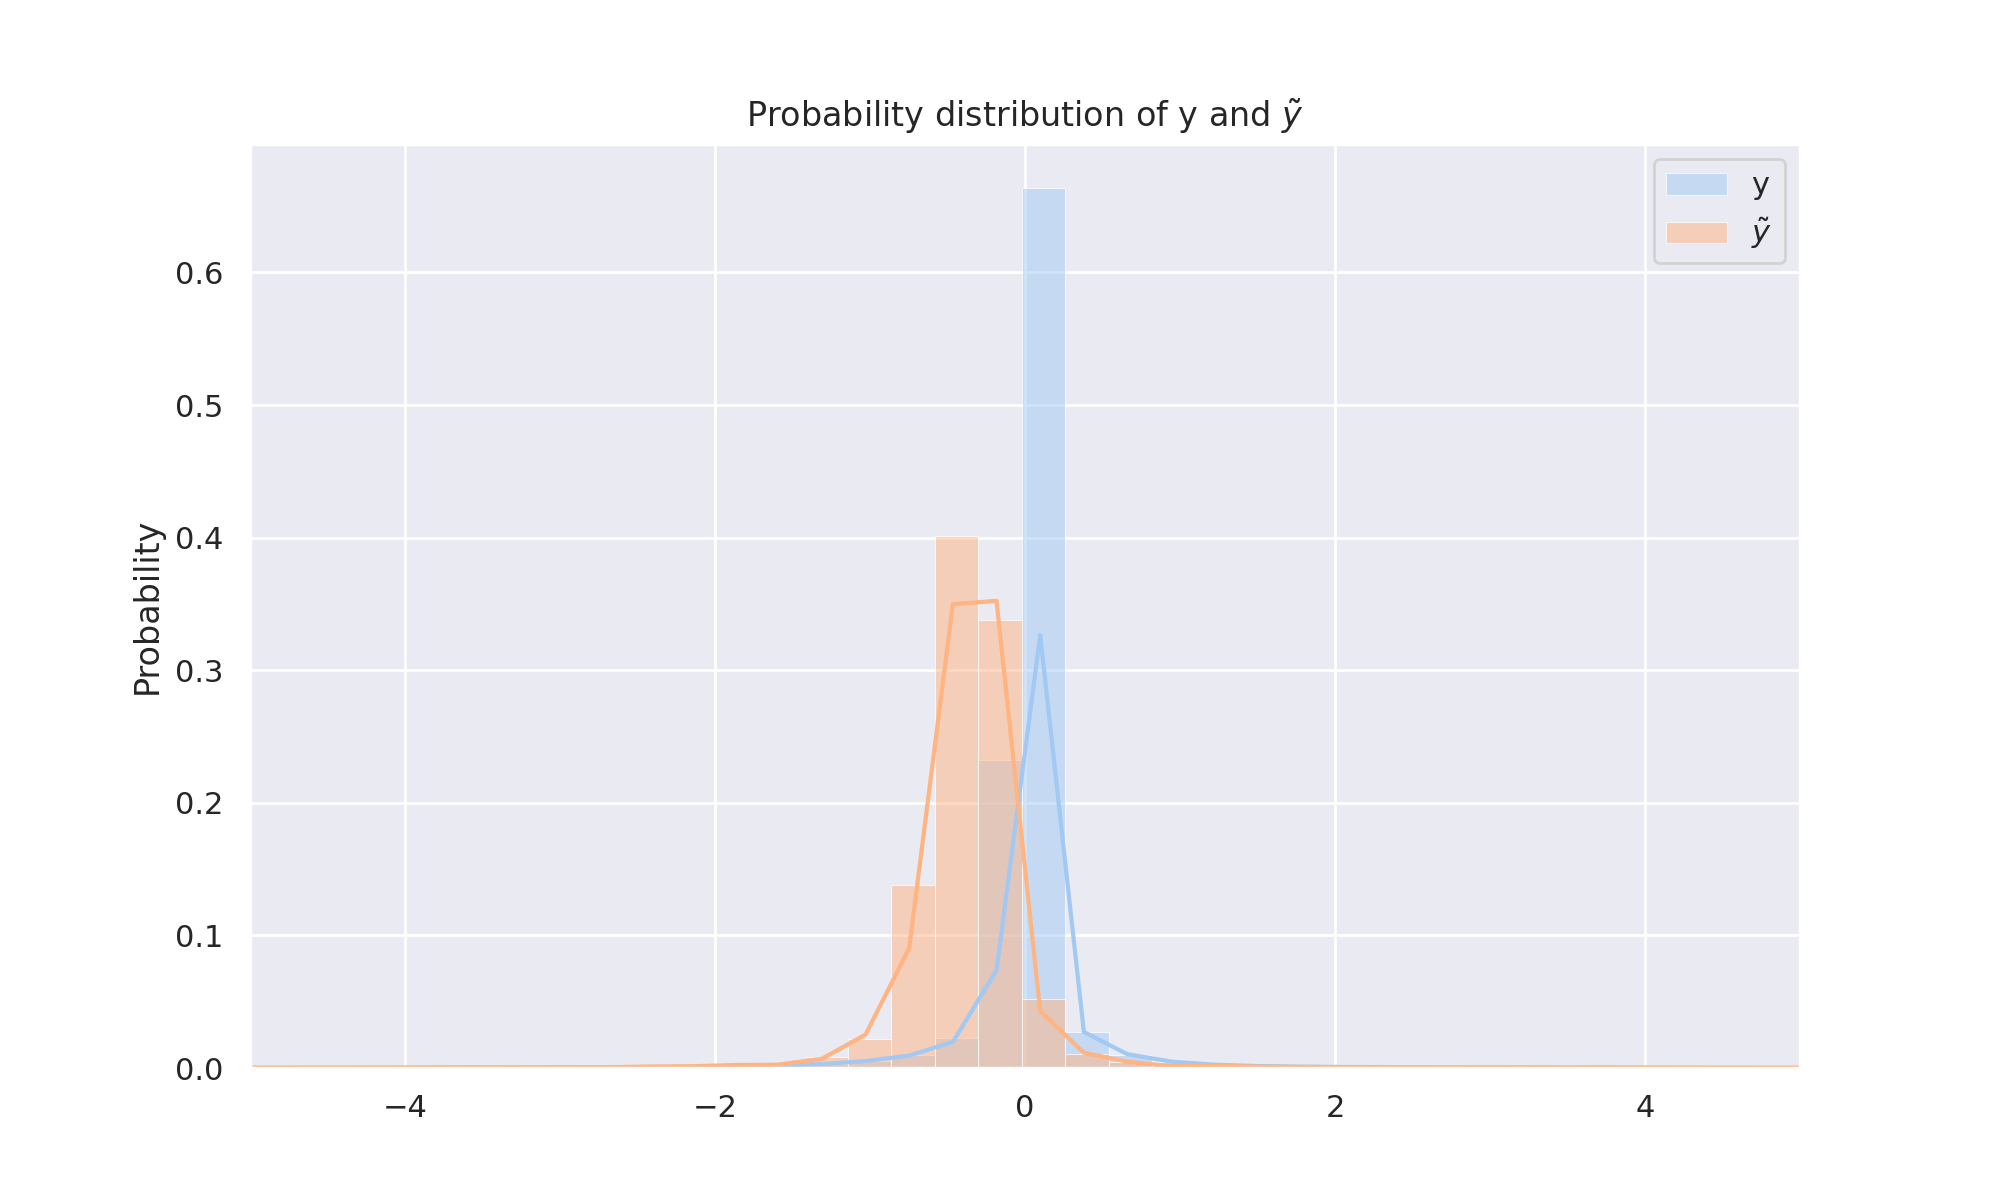
\includegraphics[width=\textwidth]{quantization_dist_50}
        \caption{Span value of $50$}
        \label{fig:quantized-y-50}
    \end{subfigure}
    \begin{subfigure}{0.5\textwidth}
        \centering
        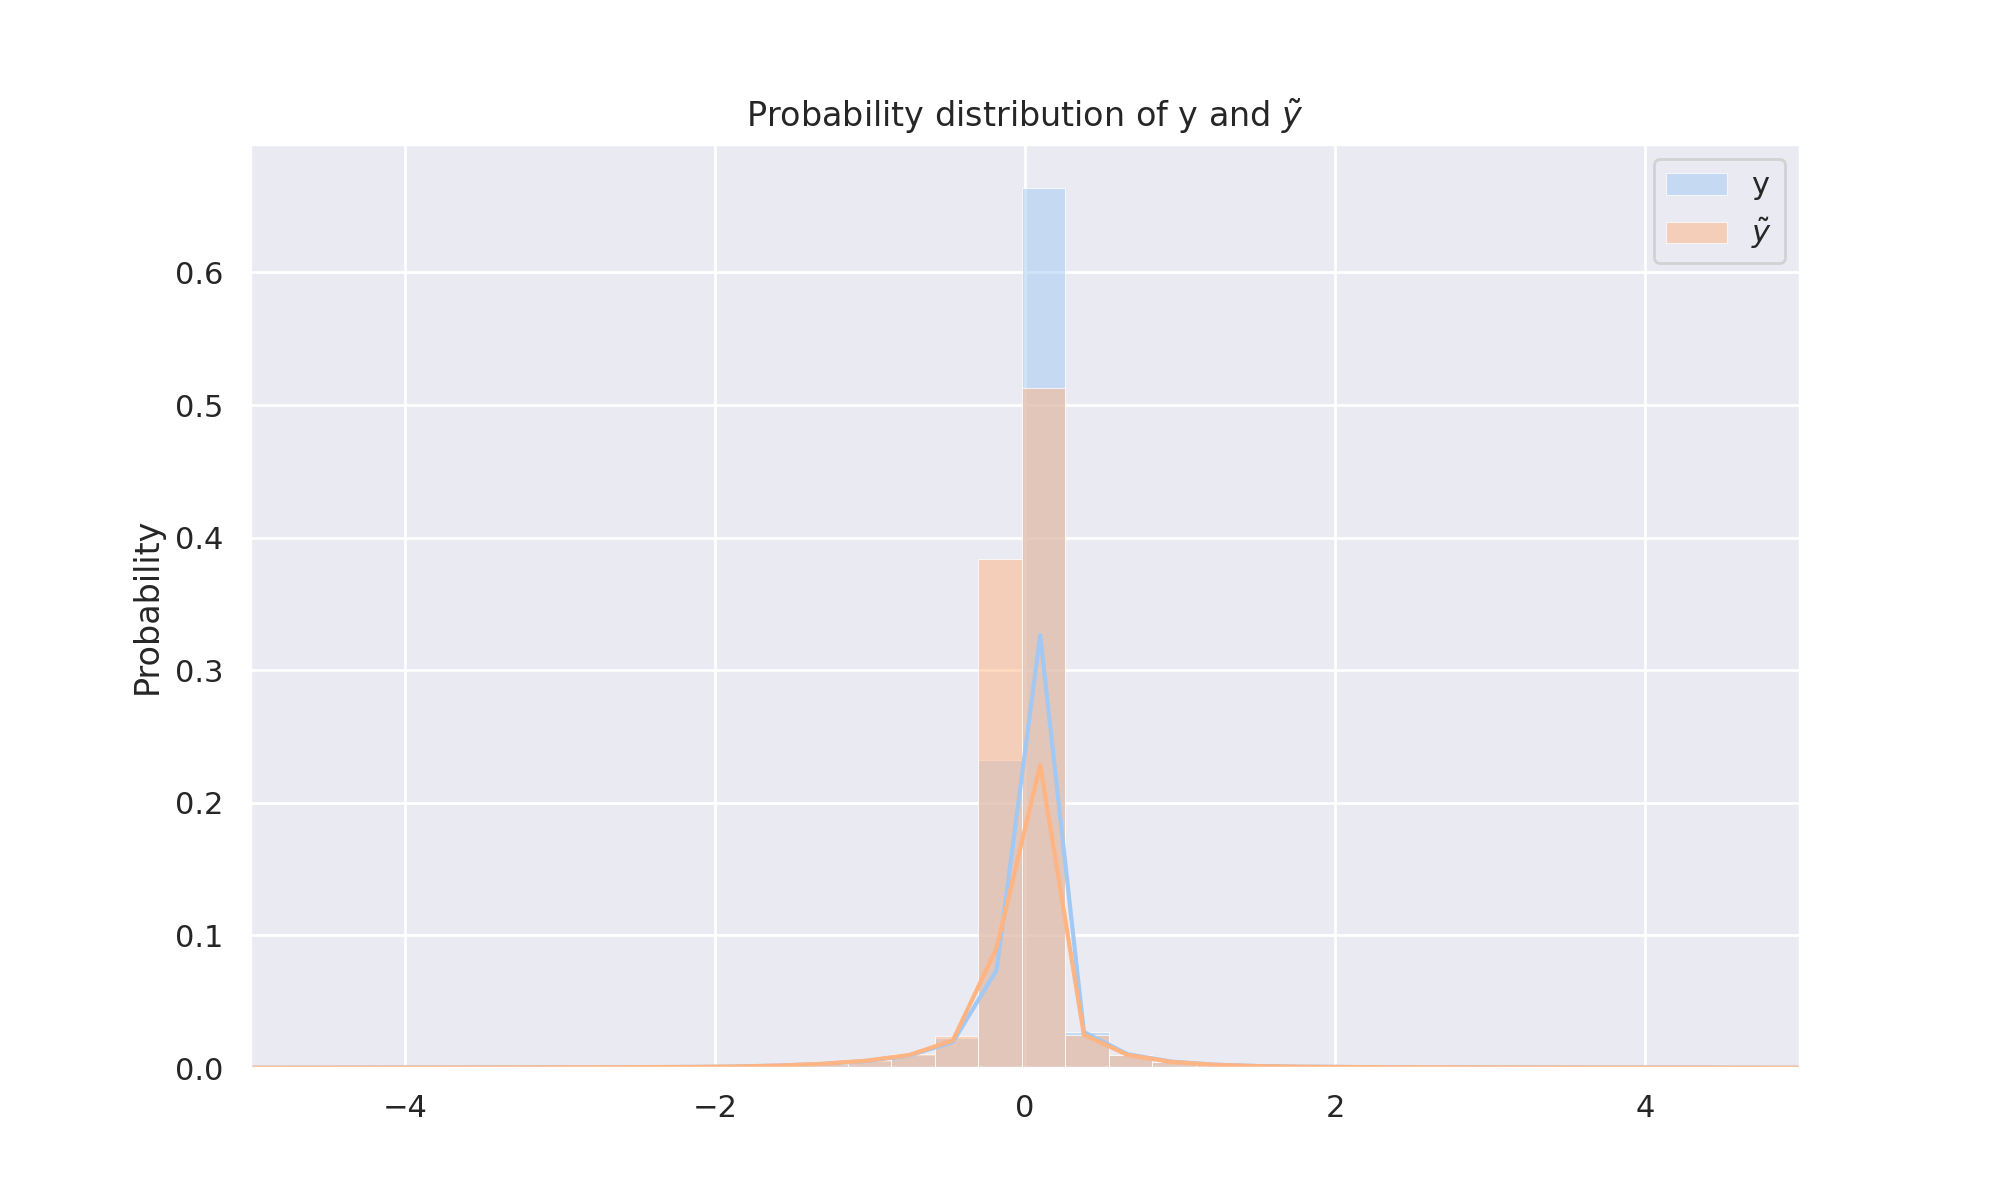
\includegraphics[width=\textwidth]{quantization_dist_1000}
        \caption{Span value of $1000$}
        \label{fig:quantized-y-1000}
    \end{subfigure}
    \caption{Latent representation $y$ and reconstructed representation $\tilde{y}$ distribution for two different span values}
    \label{fig:quantized-y}
\end{figure}

\begin{figure}
    \centering
    \begin{subfigure}{0.3\textwidth}
        \centering
        \includegraphics[width=\textwidth]{mesh/all/mitch/original00}
        \caption{Mitch}
        \label{fig:mitch}
    \end{subfigure}
    \begin{subfigure}{0.3\textwidth}
        \centering
        \includegraphics[width=\textwidth]{mesh/all/longdress/original00}
        \caption{Long dress}
        \label{fig:longdress}
    \end{subfigure}
    \begin{subfigure}{0.3\textwidth}
        \centering
        \includegraphics[width=\textwidth]{mesh/all/dragon/original00}
        \caption{Dragon}
        \label{fig:dragon}
    \end{subfigure}
    \begin{subfigure}{0.3\textwidth}
        \centering
        \includegraphics[width=\textwidth]{mesh/all/citiusp/original00}
        \caption{CITIUSP}
        \label{fig:citiusp}
    \end{subfigure}
    \begin{subfigure}{0.3\textwidth}
        \centering
        \includegraphics[width=\textwidth]{mesh/all/ipanemacut/original00}
        \caption{Ipanema Cut}
        \label{fig:ipanema-cut}
    \end{subfigure}
    \begin{subfigure}{0.3\textwidth}
        \centering
        \includegraphics[width=\textwidth]{mesh/all/fruits/original00}
        \caption{Fruits}
        \label{fig:fruits}
    \end{subfigure}
    \caption{All original vox8 point clouds}
\end{figure}
